\chapter{PR2 hardware}

\section{What's in the box}
The PR2 ships in 3 packages:

\begin{tabularx}{\linewidth}{| l | X |}
\hline      
  Robot crate & Large wooden crate which contains the PR2 itself \\ \hline
  Accessory crate & Crate which contains accessory kit, tool kit, and robot base-station \\ \hline
  Calibration target & Large checkerboard for accurate calibration of stereo cameras \\ \hline
\end{tabularx}

\subsection{PR2}
See later sections in this chapter for more detail on the PR2 robot itself or see Chapter 5 for instructions on getting it out of the crate and set up in your lab.
\subsection{Accessory kit}
\subsubsection{Wireless Joystick}
The PR2 ships with a bluetooth joystick for teleoperating the robot. The
bluetooth joystick is a
\href{http://www.sonystyle.com/webapp/wcs/stores/servlet/ProductDisplay?catalogId=10551&storeId=10151&langId=-1&productId=8198552921665411965#additionalImage1%22}{Sony
  DUALSHOCK3} (Figure~\ref{fig:ps3joy}) wireless controller. It can be charged
using any standard USB A to mini-B USB cable (one is included in the accessory kit). For more information, see the
\href{http://www.ros.org/wiki/ps3joy}{ps3joy} package at
\href{http://www.ros.org}{ros.org}.

\begin{figure}[h!]
\centering
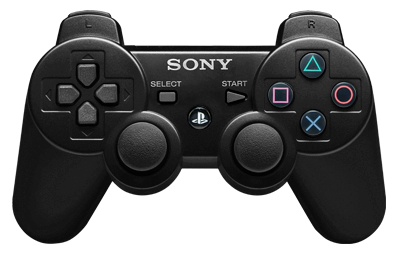
\includegraphics[scale=0.5]{ps3joy.png}
\caption{The PR2 bluetooth joystick.}
\label{fig:ps3joy}
\end{figure}

\subsubsection{Wireless run-stop}
\label{wirelessrunstop}
The PR2 comes with an
\href{http://www.omnexcontrols.com/products/portable/t50.html}{OMNEX T50}
wireless run-stop transmitter. When the red button is pressed, or the unit is
out of range, the wireless run-stop transmitter will halt the motors and put the
power system in standby mode. Note that this does not completely cut power to the robot.

\begin{figure*}[h!]
\centering
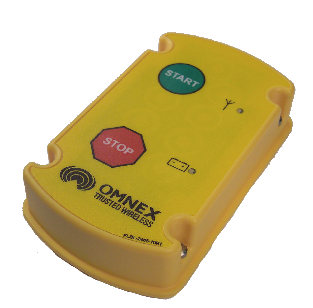
\includegraphics[width=150px]{run_stop.png}
\caption{The PR2 wireless run-stop.}
\label{fig:wirelessrunstop}
\end{figure*}

To start the wireless run-stop, press the green start button (Figure~\ref{fig:wirelessrunstop});
if this works properly, you will see a light flashing on the wireless run-stop beside the start button. While
transmitting, the wireless run-stop has a range of approximately 800 ft. The wireless run-stop is
powered by four AA batteries; the battery light will flash when the battery
charge is low and new batteries are required.

\subsubsection{Robot Power Cord and Self Plug-in Robot Power Cord}
\begin{figure*}[h!]
\centering
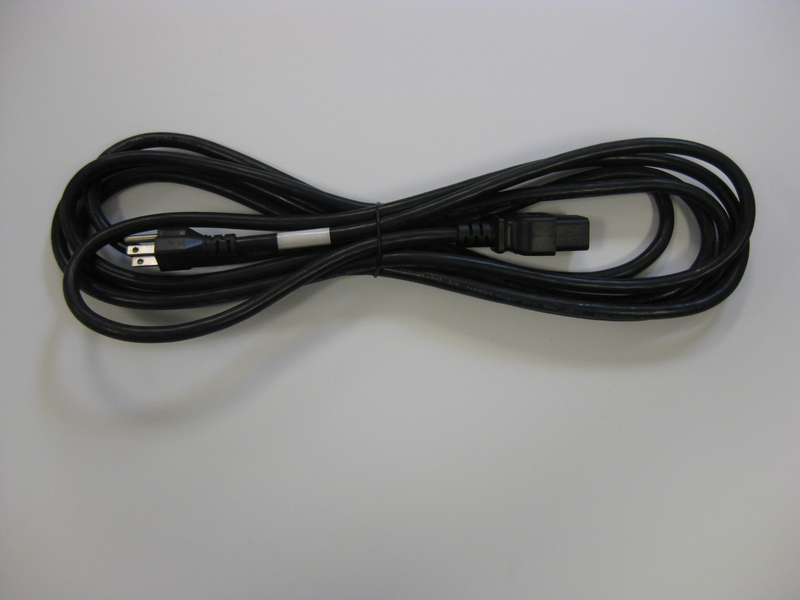
\includegraphics[width=150px]{images/long_plug.png}
\caption{Robot Power Cord}
\label{fig:longcord}
\end{figure*}
\label{longcord}

\begin{figure*}[h!]
\centering
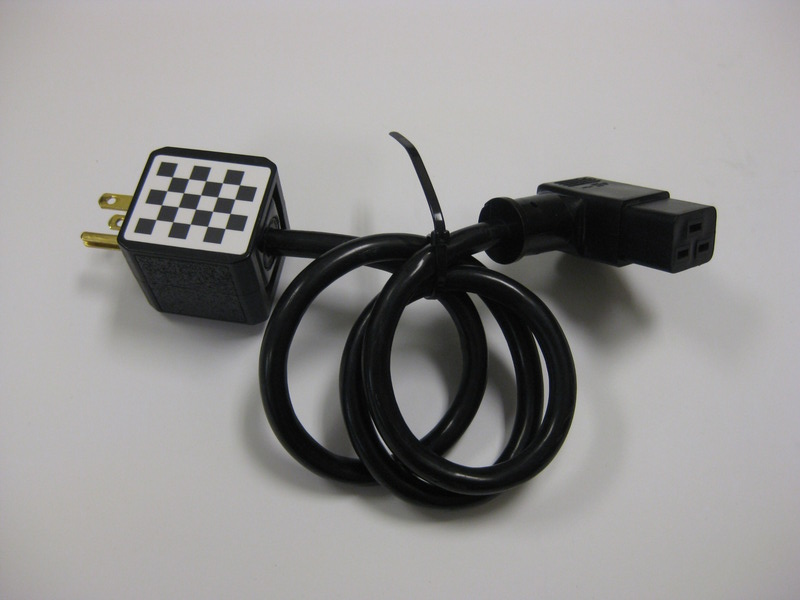
\includegraphics[width=150px]{images/short_plug.png}
\caption{Self plug-in power cord}
\label{fig:shortcord}
\end{figure*}
\label{shortcord}
To recharge the PR2's batteries, it
must be plugged into a 120V electrical outlet.  Use only the provided power
cords - many power cords and power strips have thinner conductors and cannot
safely supply the current required by the PR2.  Using inappropriate cables is
hazardous and may cause fire.  When manually plugging the robot in to re-charge, you
may use either cable.  When attepting to have the PR2 plug itself in, you must
use the shorter self-plug-in cord with attached checkerboard.  The self-plug-in
cord has magnets on the side opposite the checkerboard which should be used to
attach it to the magnetic pad on the base.

\subsubsection{Sensorized fingertips and boots}
\begin{figure}[h!]
\centering
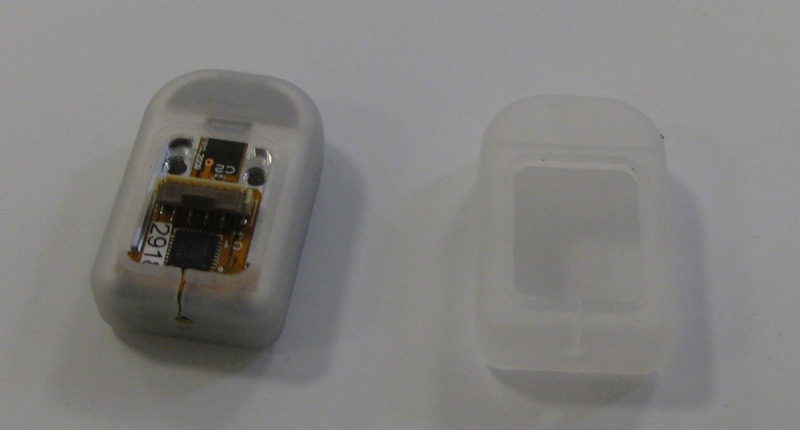
\includegraphics[width=150px]{images/fingertips.png}
\caption{Fingertip sensors and replacement boots}
\label{fig:fingertips}
\end{figure}
\label{fingertips}


The PR2 ships with sensorless
fingertips attached.  Included in the accessory kit are fingertips which have an integrated
22-element pressure sensor. These sensorized tips are easy to damage and are not as robust as
the rest of the PR2.  We provide 5 fingertip sensors (2 for each gripper, plus 1
spare), as well as 20 rubber protective "boots" which prevent the sensor from
coming into direct contact with the environment.  When using the fingertip
sensors, you should always have an undamaged boot in good condition installed
over the sensor.  Continuing to use the fingertip sensors after the rubber boot
is damaged greatly increases the chance that you will damage the sensors
themselves.  Replacement sensor tips will be available to purchase from Willow Garage.  See the support site at \href{http://support.willowgarage.com}{support.willowgarage.com} for more information.

\subsubsection{Small calibration target}
\begin{figure}[h!]
\centering
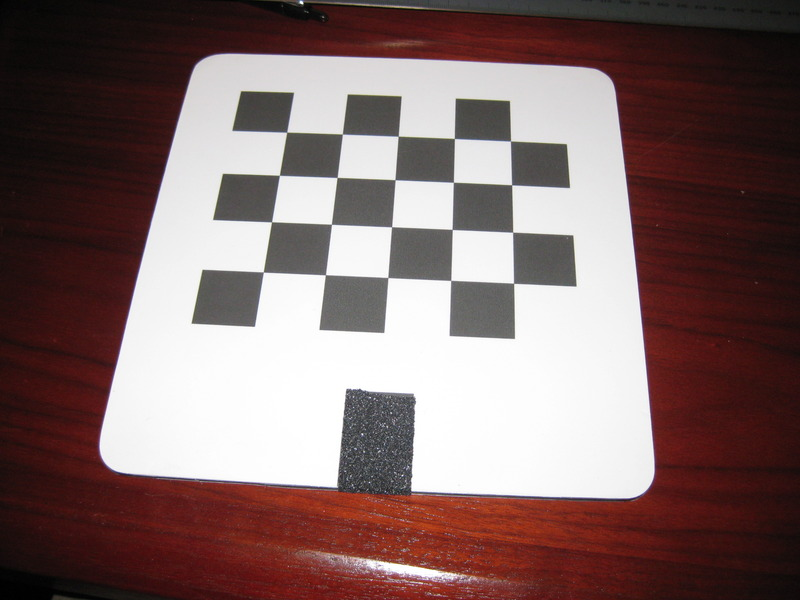
\includegraphics[width=150px]{images/hand_checkerboard.png}
\caption{Small calibration target}
\label{fig:hand_checkerboard}
\end{figure}
\label{hand_checkerboard}

This small hand-held calibration target, which looks
like a checkerboard, is used for the PR2 self-calibration.  The robot holds the
checkerboard in one gripper and uses it to calibrate the arms, the head, the
cameras, and the tilting laser together.  The squares on the board are 25mm in each direction.

\subsection{Large calibration target}
The large calibration target which ships with the robot looks like a
checkerboard 1" thick and approximately 3 feet square.  This is the
recommended calibration target to use for calibrating the intrinsics of the
stereo cameras on the robot.  The robot ships with stereo cameras already
calibrated, but you may need to re-calibrate after shipping, and occasionally as vibration and
thermal effects change the parameters over time.  The squares on the board are 108mm in each direction.
Since the flatness of the board is critical to the accuracy of the calibration, please store this where it will not warp.

\subsubsection{User Manual}
Printed version of this document.

\subsection{Toolkit}
\begin{figure}[h!]
\centering
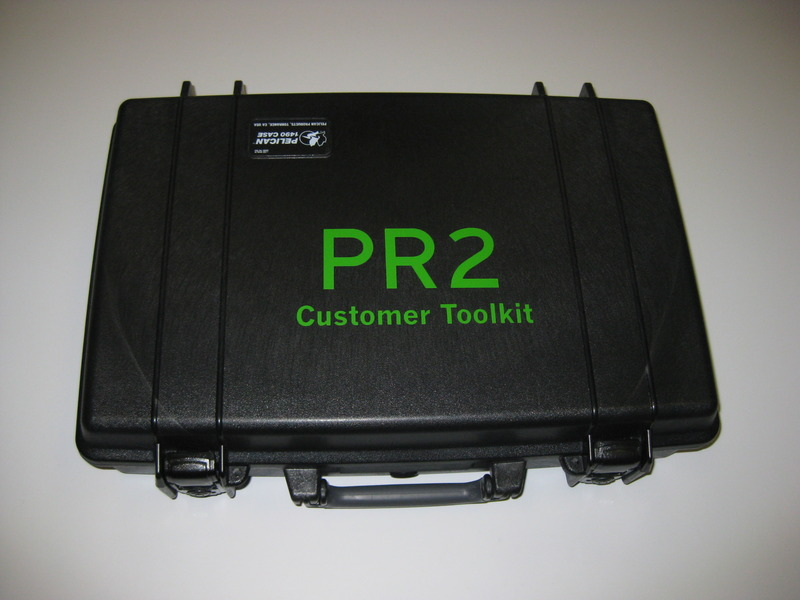
\includegraphics[width=150px]{images/toolkit.png}
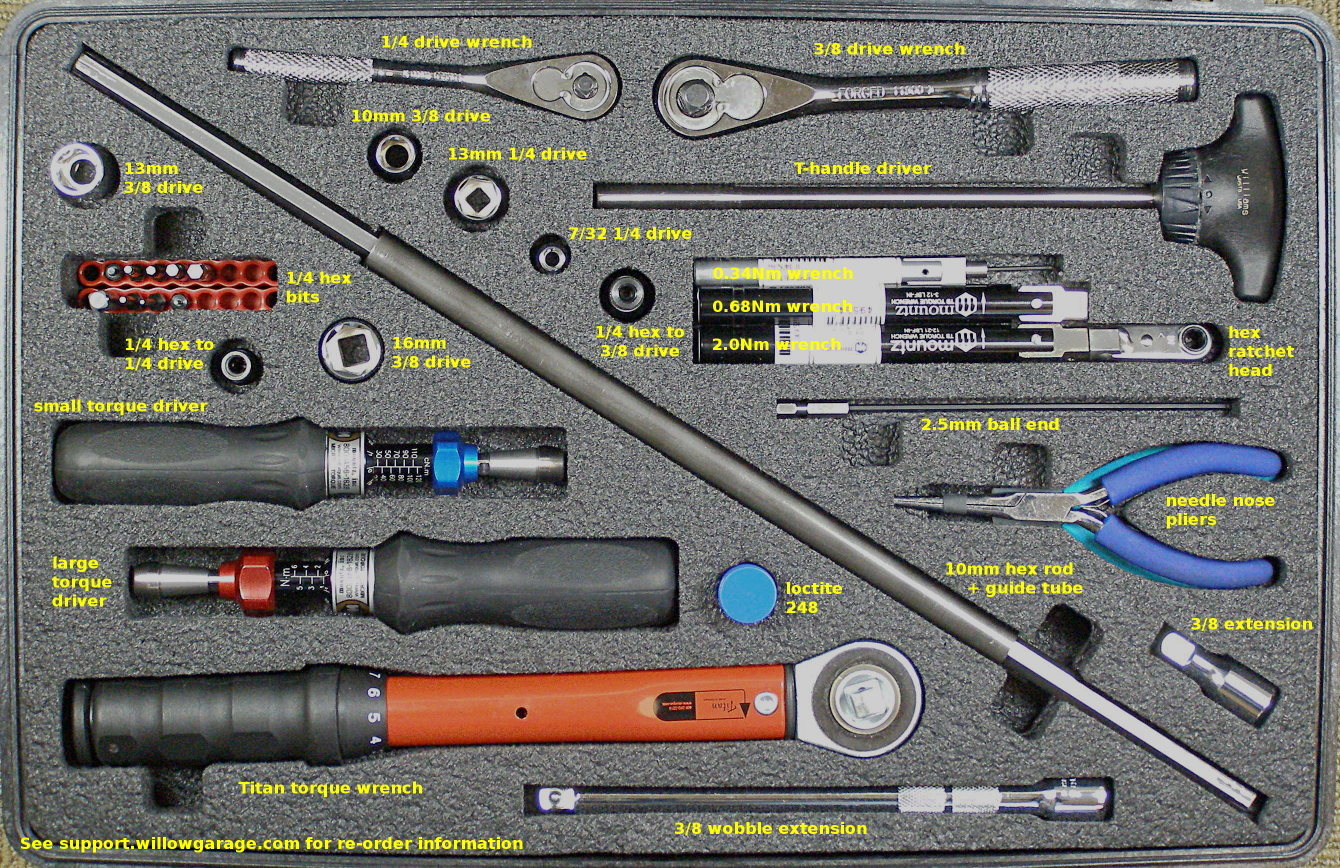
\includegraphics[width=150px]{images/toolkit_layout.png}
\caption{PR2 toolkit}
\label{fig:toolkit}
\end{figure}
\label{toolkit}
A toolkit is provided with the PR2.  To avoid damaging the robot or injuring yourself, you should always use these tools and follow the Repair and Replacement procedures at support.willowgarage.com when performing any hardware maintenance on the robot.


\subsection{Base-station computer}
\begin{figure}[h!]
\centering
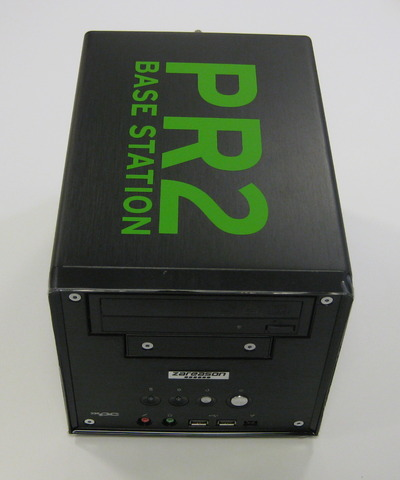
\includegraphics[width=150px]{images/basestation.png}
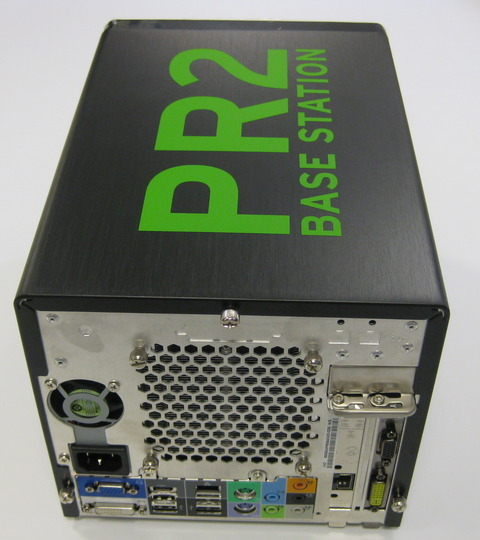
\includegraphics[width=150px]{images/basestation_back.png}
\caption{PR2 Base-station computer}
\label{fig:basestation}
\end{figure}
\label{basestation}

The base-station computer ships
without a monitor, keyboard, or mouse.  See chapter 4 on computers for more information on how to configure your base-station.

\section{Mechanism}
PR2 is a 32-dof mobile manipulator with a mobile base, two arms, and a variety
of sensors on a pan-tilt head.

\subsection{Terminology}
We talk about the robot kinematics using the concepts of joints, links, frames,
actuators, and transmissions.  Each of these is defined and represented in code,
as well as having a unique name.  In general, a single joint will have an
actuator and a transmission and will connect two links together.  A link is a
rigid body in the kinematic tree, and will have a coordinate frame, but not all
frames are associated with links.  We allow "fixed" joints, so some rigid bodies
that could be considered one link are considered to be two links rigidly joined
together.  This is done mostly at locations where there is a physical interface
between components.

\begin{description}
\item[Link] We consider a link to be a rigid body within the robot.  It
  generally has geometry to define visual and collision-space representations,
  has inertial properties, and has a name.  The links for the PR2 are defined in
  the "URDF" description that can be found in the pr2\_description package.
\item[Frame] Frames are geometric entities that represent coordinate frames in
  space.  Every link has an associated frame, but we also use frames to
  represent other things, such as the optical frame of a camera, the global map,
  or the location of a detected object.  Frames are always defined relative to
  one another, and relationships and transformations between them are tracked
  using the tf package.
\item[Joint] Joints are considered part of the robot, and define the
  relationship between links.  The joints for the PR2 are defined in the URDF
  description that can be found in the pr2\_description package.  The PR2 has
  mostly rotational joints, but the torso is translational, and there are also a
  number of "fixed" joints used to represent the notion that two links are part
  of the same rigid body.  Rotational and translational joints are generally
  represented in the same way in the system, and we refer to joint "effort"
  instead of force or torque, as well as using position, and velocity to
  represent both linear and angular movement.
\item[Actuator] The motor/encoder units in the PR2 are explicitly modelled as
  "actuators".  The actuator model treats them as torque sources with position
  measurement.  The details of the actuator model (e.g. the motor torque
  constant or max current), as well as the name of the actuator, are stored on
  the motor controller boards.
\item[Transmission] We use transmissions, also defined in the URDF robot
  description, to represent the mapping between actuators and joints.  They map
  actuator position into joint position (meters or radians), and map from
  commanded joint efforts (torques or forces) to actuator efforts.  In most
  cases in the robot this is a linear mapping between one joint and one actuator
  that just defines a reduction, but in the wrist we have 2 motors controlling
  two joints in a cross-coupled manner, and in the gripper the mapping from
  motor rotation to gripper position is non-linear.
\end{description}

In general, the names for a link and the associated frame will be similar
(e.g. r\_forearm\_link and r\_forearm\_frame), and the names for an actuator, a
transmission, and the associated joint will be similar
(e.g. r\_elbow\_flex\_motor, r\_elbow\_flex\_trans, and r\_elbow\_flex\_joint).
For components such as arms and casters that are included in the robot in
multiple locations, we use a short prefix to indicate which location we are
referring to

\begin{tabular}{| l | l |}
\hline
  l\_ & left (from the robot's perspective) \\ \hline
  r\_ & right \\ \hline
  fr\_ & front right \\ \hline
  fl\_ & front left \\ \hline
  bl\_ & back left \\ \hline
  br\_ & back right \\ \hline
\end{tabular}

\begin{figure}[!h]
\centering
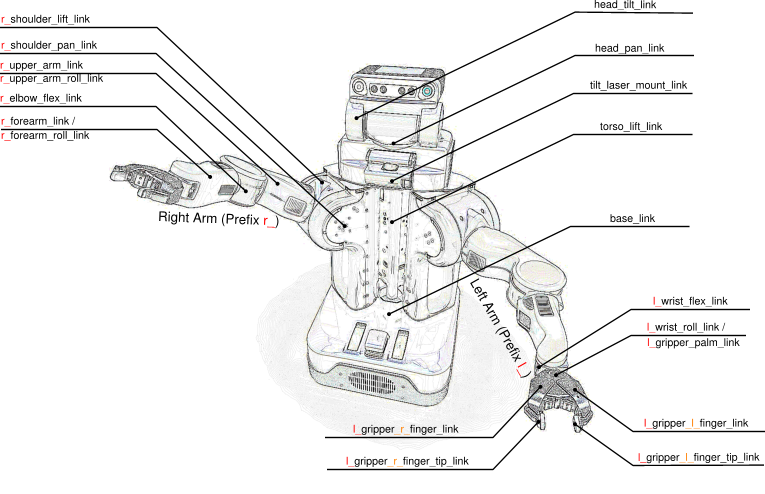
\includegraphics[scale=0.6]{urdf_links.png}
\caption{The PR2 URDF Link Naming Scheme.}
\label{fig:urdf_link_names}
\end{figure}
\begin{figure}[!h]
\centering
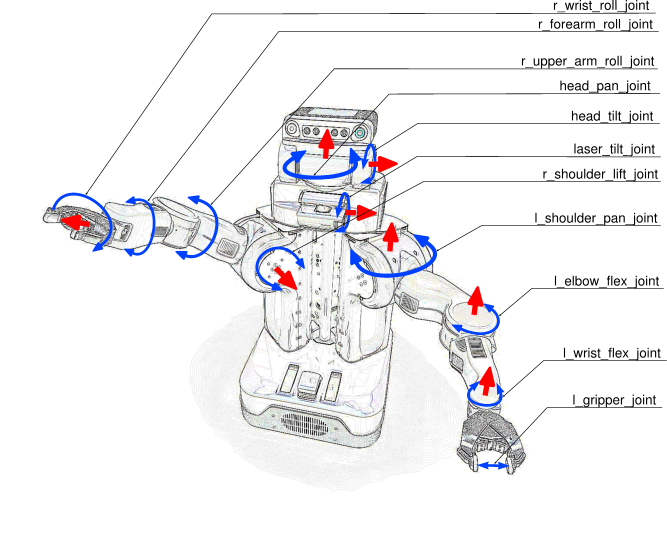
\includegraphics[scale=0.6]{urdf_joints.png}
\caption{The PR2 URDF Joints Naming Scheme.}
\label{fig:urdf_joints}
%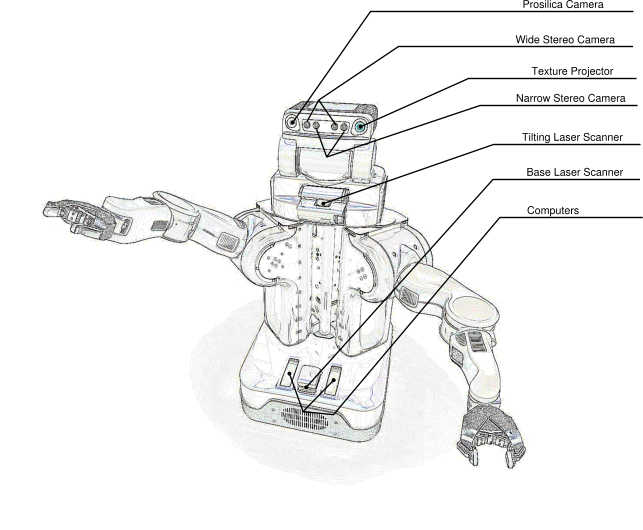
\includegraphics[scale=0.4]{urdf_sensors.png}
%\caption{The PR2 Sensors.}
%\label{fig:urdf_sensor}
\end{figure}

\subsection{Links and Joints}
By component, below is a list of the links and joints in the PR2:
\subsubsection{Base-Body-Spine}
The base-body-spine assembly of the PR2 has only one joint - the prismatic {\bf
  torso\_lift\_joint} which moves the torso up and down relative to the base.
The {\bf base\_link} holds the rear panel with electrical/network connections,
the computers, and the battery system, as well as bolting directly to the
casters.  The {\bf torso\_lift\_link}, which moves up and down, contains the
speaker, and the IMU, as well as serving as the attachment point for both arms
and for the head.
\subsubsection{Head}
The pan-tilt head which holds the wide and narrow stereo cameras, the 5
mega-pixel camera, and the texture projector is made up of two links - the {\bf
  head\_pan\_link}, connected to the torso by the {\bf head\_pan\_joint}, and
the {\bf head\_tilt\_link}, connected to the pan link by the {\bf
  head\_tilt\_joint}.  The sensors are all attached to the tilt link.

The upper Hokuyo laser range-finder is mounted to the {\ laser\_mount\_link},
which is tilted up and down by the {\bf laser\_tilt\_mount\_joint}
\subsubsection{Casters}
Each robot has four steered and driven casters, one at each corner of the base.
The casters are refered to as front right, front left, back right, and back
left.  They are named according to the above table of location prefixes ({\bf
  fr\_}, {\bf fl\_}, {\bf br\_}, and {\bf bl\_}).  Each caster consists of a
rotation joint {\bf location\_caster\_rotation\_joint}, which rotates or steers
the body of the caster, called the {\bf location\_caster\_rotation\_link},
around a vertical axis.  Attached to the body of the caster are two parallel
driven wheels, whose drive joints are {\bf location\_caster\_r\_wheel\_joint}
and {\bf location\_caster\_l\_wheel\_joint}.

\subsubsection{Arms}
The arm has 7 degrees of freedom.  Starting from the attachment to the torso,
the first joint is the {\bf location\_shoulder\_pan\_joint} which rotates the
{\bf location\_shoulder\_pan\_link}, or shoulder turret, around a vertical axis.

The shoulder turret contains the springs that store energy to counterbalance the
mass of the rest of the arm.  Two degrees of freedom, the {\bf
  location\_shoulder\_lift\_joint} and {\bf location\_upperarm\_roll\_joint}
attach the {\bf location\_upper\_arm\_link} to the shoulder.

The upper arm contains the counterbalance bar, which is a large steel bar that
attaches to the counterbalance attachment and transmits the counterbalance
forces into the structure of the arm.  The upper-arm also contains motors for
the {\bf location\_elbow\_flex\_joint} and {\bf location\_forearm\_roll\_joint},
which connect the forearm to the upper-arm.

The forearm ({\bf location\_forearm\_link}) contains a 640x480 color camera that
can always see the gripper, as well as the two motor which drive the {\bf
  wrist\_flex\_joint} and the continuous {\bf location\_wrist\_roll\_joint} that
attaches to the gripper.

\subsubsection{Grippers}
The gripper consists of a central palm link called the {\bf
  location\_gripper\_palm\_link} which is rigidly fixed to the {\bf
  location\_wrist\_roll\_link} and has a single actuated degree of freedom.  The
motor in the gripper drives the 4 joints of the gripper together to result in
parallel motion of the fingertips.  The parallel distance between the gripper
tips is treated as a translational joint, called {\bf location\_gripper\_joint}
that can be controlled.  The four rotational joints in the hand which are
constrained to move together are also modelled as joints which can be observed
but not controlled.  The gripper also contains a 3-dof accelerometer and an LED
which can be turned on and off to assist in calibration or finding the location
of the gripper in camera images.

\subsubsection{Additional Information}
A CAD approximated kinematic and inertial description of the PR2 can be found in
the \href{http://www.ros.org/wiki/pr2\_description}{pr2\_description} package.
This package uses a robot specific Extensible Markup Language (XML) and Document
Object Model (DOM) representation called
\href{http://www.ros.org/wiki/urdf}{Uniform Robot Description Format(URDF)}, which can
be converted or exported to other formats such as COLLADA.

%\TODO{Include updated tables of joint limits, torques, home positions, etc.}

\subsection{Drivetrains}
The joints in the PR2 are all actuated with brushed electric motors, and all
position sensing is done with optical incremental quadrature encoders.  Except
where noted, each joint has an optical sensor (interrupt or reflective) which is
used at startup to identify a home position.  Once the home position is
identified, the incremental encoders are used to track motion.  All drivetrains
in the robot have positive-engagement drives (gears or belts), and the motor
controllers monitor for encoder errors, so there should not be any drift in
measured position over time, although the repeatibility of the calibration
sensors may cause minor differences in position sensing between runs.

Velocity estimates are made by differentiating the position sensors at 1ms, so the
quantization of the encoders produces noise in the velocity signal, which is
especially significant at low speeds.

Torque estimates are made by measuring the commanded current of the motor and
using the values of the torque constant from the datasheet together with the
model of the transmission.  These transmission models assume 100\% efficiency,
and accuracy of torque estimates and commands is limited by the friction in the
drivetrain, so joint torque accuracy should be characterized where you are
relying on it.

\begin{description}
\item[Torso Drivetrain] The torso is driven up and down on a linear rail by a
  combination of a gas spring, which supports most of the weight of the torso,
  and a lead-screw which is driven via an RE40 motor with 113:1 gearhead
  connected to a continuous belt drive with a 5:1 reduction.  As a result of the
  force from the gas-spring not being constant over the range of travel, the
  lead-screw may be loaded up, down, or neutrally as different points of travel
  of the torso.  Position sensing of torso lift is done via optical encoder on
  the back of the motor, so any backlash in the lead-screw, belt, or gearhead is
  not sensed.  The torso joint is quite low efficiency, so commanding large
  forces (in the range of 1000 newtons) will be required to move the torso.  The
  maximum speed of the torso lift joint is limited by the thermal rating of the
  lead-screw nut.  Driving the torso lift link faster than the velocity limit
  will cause permanent damage to the lead-screw assembly.  Similary, driving at
  the safety limit but with excessive load Because of the large reduction, the
  torso lift link is capable of exerting high forces, so take care

\item[Head Drivetrains] The drivetrains for the head pan, head tilt, and laser
  tilt are all fairly similar.  Since precise pointing of sensors is important,
  all three of these joints have 10,000 count encoders mounted in the drivetrain
  after the major sources of potential backlash (gears).  The laser tilt axis is
  driven directly by the motor, through the encoder, and then via a belt-drive.
  The head pan and tilt are both driven from the motor through a gearset
  (planetary gearhead for the tilt joint and external spur gears for the pan
  joint).  The encoder is mounted on the shaft after the gearset, and then a
  belt drive is used for the final stage reduction.  These drivetrains are all
  high-efficiency and capable of very high velocities.  The software velocity
  and position limits on these joints are important to prevent hard collisions
  with the joint stops, which will cause damage to the hardware (espially to the
  sensors).  If the mass of the head is changes significantly, the pan and tilt
  link gains may need to be re-tuned.

\item[Caster Drivetrains] The three joints in each caster have basically the
  same drivetrain, which is a Maxon amax-32 motor with a gearhead and a
  continuous belt output.  Position sensing is done via an encoder on the back
  of the motor.  The drivetrain is efficient enough to be easily backdriveable.
  To rotate the caster, all three motors work together (the rotation motor
  drives the rotation, and the two wheels drive in opposite directions to
  provide additional forces.  To drive, the two wheel motors rotate in the same
  direction and the rotation motor helps to keep them aligned in the proper
  direction.

\item[Arm Drivetrains] The first four degree of freedom in the arm (shoulder
  pan, shoulder lift, upperarm roll, and elbow flex) are all driven with RE40
  motors that have single-stage planetary gearheads which output to a toothed
  pulley that runs on a belt.  These belts all have terminations at either end
  of a capstan on the moving link, which is how the torque is transmitted.  The
  terminations are also the way that these belts are tensioned, and propoer belt
  tensioning is important to prevent backlash (which can come from extra slack
  in the belt), friction (which can come from extra tension in the belt), and
  excess wear (which can come from a belt which is too tight, too loose, or just
  misaligned).  The position is measured via an optical encoder on the back of
  the motor, so the backlash of the gearhead and the stretch of the belt both
  contribute to the error in the sensed position.  Velocity limits are important
  on these joints to prevent motor damage from running over speed, as well as to
  prevent rapid decelleration which can damage the motor, gearhead, and belt.

These drivetrains are all fairly high efficiency, which means they can be
backdriven.  This is made possible by the low force requirements on those joints
due to the arm counterbalance.  The counterbalance uses a system of springs and
linkages to compensate for the effect of gravity on the upper arm and forearm
links.  The compensation should be effective throughout the range of motion of
the first four links of the arm.

\item[Arm Counterbalance] Although not an actuated drivetrain the arm counter
  balance is one of the more complicated mechanisms on the PR2. Inside of the
  shoulder turret there are two springs.  These springs are attached to belts
  which run over cams and provide a uniform downward force.

In the upper arm there is a four-bar linkage which transmits the torque through
to the shoulder lift joint, upper-arm roll joint, and elbow flex joint.  As the
arm moves through its configuration space the linkage changes the amount of
leverage with which the counterbalance is pulling which compensates for the
effect of the mass of the arm in difference configurations.

\item[Wrist Drivetrains] The forearm roll joint is driven by a motor in the
  upperarm with a planetary gearhead and external spur gear.  Position is
  measured via an optical encoder on the back of the motor.  Because of the
  higher gear reduction, the efficiency and backdriveability of this joint is
  not as good as that of the first four joints of the arm.

The wrist flex and roll use a differential drive between two motors.  If the
motors are turned in the same direction the wrist rolls, if they are turned
oposite the wrist flexes.  The differential bevel gears are attached after a
standard encoder, motor, gearhead assembly.


\item[Gripper Drivetrain] The gripper consists of two fingers with two joints
  each.  Within each finger, a four-bar linkage constrains the two joints to
  move together so that the fingertips remain parallel.  The two fingers are
  constrained together with a sector gear that meshes between the first
  phalanges of the two fingers.  The motion of the fingers is driven by a motor
  which drives a lead-screw in the palm of the hand.  This lead-screw is
  embedded in the four-bar linkage so that the rotation of the motor has a
  nonlinear relationship to the movement of the joints.  The gripper can be
  back-driven when significant force is applied.  Unlike all other
  non-continuous joints in the system, the gripper has no calibration flag.
  Initial homing is done by closing the gripper until it gets blocked and then
  treating that position as a zero point.  This means that the gripper is unable
  to detect if it has miscalibrated on startup.

\end{description}


\subsubsection{Home Pose}
In order to describe the PR2 robot pose and joint positions in a consistent
manner, a {\bf home pose} of the robot has been defined.  At the home pose,
all joint-angles are considered to be at zero.  In the home pose the casters
are facing straight ahead, the arms are straight ahead in front of the body,
the grippers are closed, the tilting laser is level, and the head is centered
and flat.  For most joints the calibration reference point is not at the home
pose, or zero position, and the URDF contains the offsets between the flag
positions and the home position.

\subsubsection{PR2 Coordinate System}
\label{sec:pr2_coordinate_system}
The coordinate frames for all links of the PR2 are defined to be aligned with
 a world coordinate frame of positive z-axis up, positive x-axis forward, and
positive y-axis robot-left when the PR2 is in the home pose.  All joint angle conventions
are chosen so that at the home position, positive motion of the joint causes positive
motion around one of the positive axes of the world coordinate system.

\subsection{Motion control}

\begin{figure}[h!]
\centering
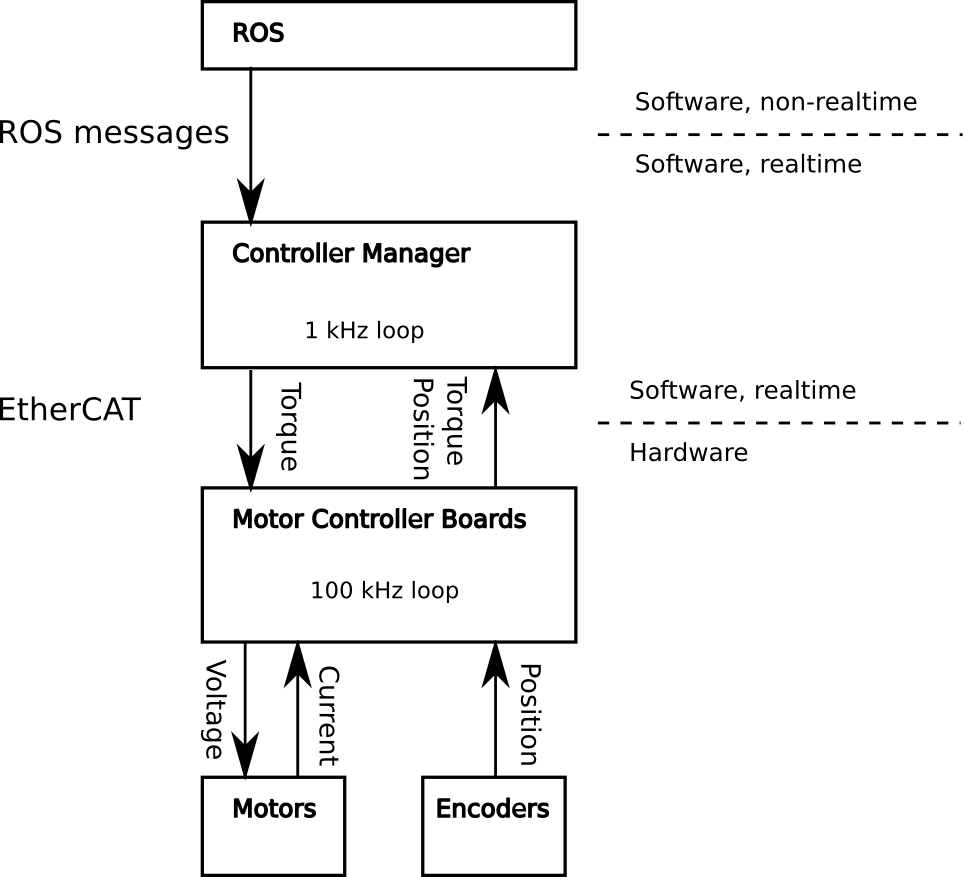
\includegraphics[width=290px]{images/mechanism_control.png}
\caption{Motion control layout.}
\label{fig:motion_control}
\end{figure}


\subsubsection{Motor controller boards}
Each motor/encoder on the PR2 has its dedicated \emph{Motor Controller Board}
(MCB). The MCB detects and counts transitions in the encoder signal, measures
the motor current, and commands the voltage going to the motor. Each MCB runs a
PI-control loop to control the motor current to a desired value, by commanding
the motor voltage. This control loop is closed at 100kHz on an FPGA on the MCB.  A
shared etherCAT realtime Ethernet link with the first computer allows all MCBs
 in the PR2 to communicate with the main computers with deterministic timing.

Each MCB has the following inputs and outputs:
\begin{description}
\item[Encoder input] Each MCB can read quadrature incremental encoder input.  In proper operation, this should never skip or drift.
\item[Power input] Each MCB is connected to the raw battery-power bus, and using the circuit breakers you can switch between "enabled", which provides 44-80VDC
to the MCB and allows it to drive the motor, "standby", which provides 18VDC to the MCB and allows it to continue to communicate and read sensors but
doesn't allow driving the motors, and "disabled", which turns off power the the MCB altogether.
\item[Digital input] Each MCB has a digital input which is used for detecting the flags at the calibration positions on power-up.  The MCB internally latches the encoder counts at the time that the digital input transitions from high to low and from low to high, which accurate detection of calibration flag positions.
\item[Digital output] Each MCB has a digital output.  On the gripper, this is used to control the LED mounted in the hand.
Elsewhere in the robot, this is used to generate synchronization pulses which allow synchronizing the cameras, the projector,
and the motion control systems together precisely.
\item[Motor output] Each MCB can drive a single brushed DC motor.  The MCB drives the output with an H-bridge and uses a current-measurement to do closed-loop current control on the motor.
\item[SPI] There are two SPI ports which are only available on the gripper MCBs and which are used to connect to the fingerip sensors.
\end{description}

\subsubsection{Realtime loop}
The realtime loop for the PR2 is a single process, which can be found in the pr2\_ethercat package.  At runtime, the node is called {\bf realtime\_loop}.

This process uses the RT\_PREEMPT extensions to the Linux kernel to run as a hard realtime process, with a cycle time of 1ms, and performs both controller update computations and communication over EtherCAT with the MCBs.  Non-realtime threads within the same process are used to communicate over ROS to publish diagnostics, configure controllers, and otherwise control the behavior of the PR2's motion-control system

\subsubsection{Controller manager}.  
Within the realtime loop, the controller update is dealt with by a ROS component which contains both realtime and non-realtime functionality,
called the \emph{Controller Manager}.  Controlle Manager has an update step which
is called by the realtime loop at 1khz which receives measured motor torques and positions and sends
desired motor torques for the next cycle.

The Controller Manager includes the joint-limit safety code that enforces position, velocity, and torque limits
which are necessary to keep the PR2 from damaging its hardware.  In addition, it has a
dynamic plugin loading mechanism that allows shared libraries containing realtime controllers to be loaded
and executed inside the 1kHz realtime loop.

\subsection{Mechanical specs}

Before undertaking any new or risky operations with your PR2, please consult
these mechanical specifications. Do not operate the PR2 outside of these
specifications. If you have any questions about your PR2's specifications,
please contact Willow Garage Support.

\subsubsection{Environmental specs}

The PR2 is an indoor, household robot. Operating outside this type of environment could cause damage to the PR2, and  injury or death to operators.

\paragraph{Water}

The PR2 has not been tested for any type of contact with water or any other
liquid. Under no circumstances should the PR2 come in contact with water from
rain, mist, ground water (puddles) and any other liquid. Water contact can cause
damage to the electrical circuitry and the mechanism.

\paragraph{Temperature and Humidity}

Temperature testing of the PR2 has allowed the unit to run between 15 and
35C. Towards the upper end of this range, above 30C, you may experience decreased performance of the batteries. Temperatures outside of this range can cause malfunctions in the PR2 power system and instruments. The PR2 has been tested in high humidity, but under no
circumstances should condensation be allowed to form on the mechanism.

\paragraph{Drive Surface}

The drive surface of the PR2 must be capable of supporting the entire weight of
the PR2, about 450 pounds (220 kgs). If the surface is too soft, the PR2 can get
stuck and fail to drive. A commercial carpet or tile is recommended.

\paragraph{Incline Surface}

The PR2 is ready for ADA-compliant ramps, which are at 1/12 slope. Ramps that
are steeper than a 1/12 slope are unsafe and may be a tip over hazard.

\paragraph{Other Environmental Specs}

\begin{itemize}
\item UV exposure should be minimized. UV radiation can damage the PR2's skin
\item Dust and dirt can clog air filters
\end{itemize}

\subsubsection{Forces and torques}

Joint position, velocity, and force limits are implemented in the PR2's URDF
file, in the ``/etc/ros/$<$distro$>$/urdf/robot.xml" file on your PR2. These joint limits
control the range of travel of the mechanism, the allowable velocity to prevent
overtravel. These limits are enforced by pr2\_controller\_manager, and are
designed to prevent poorly commanded control efforts from damaging the PR2 and
harming operators.

The limits below are from the PR2 URDF file. If a velocity or torque limit is
not specified, no value is enforced by pr2\_controller\_manager.

\begin{tabular}{l*{2}{c}}
Joint  & Velocity (rad/s or m/s) & Torque (Nm or N) \\
\hline \hline
$\ast$\_caster\_rotation\_joint        & -     & -  \\
$\ast$\_caster\_wheel\_$\ast$\_joint   & -     & -  \\
torso\_lift\_joint                     & 0.013 & 10000 \\
laser\_tilt\_joint                     & 10.00 & 0.65  \\
head\_pan\_joint                       & 6.00  & 2.65  \\
head\_tilt\_joint                      & 5.00  & 15.00 \\
$\ast$\_shoulder\_pan\_joint           & 2.10  & 30.00 \\
$\ast$\_shoulder\_lift\_joint          & 2.10  & 30.00 \\
$\ast$\_upper\_arm\_roll\_joint        & 3.27  & 30.00 \\
$\ast$\_elbow\_flex\_joint             & 3.30  & 30.00 \\
$\ast$\_forearm\_roll\_joint           & 3.60  & 30.00 \\
$\ast$\_wrist\_flex\_joint             & 3.10  & 10.00 \\
$\ast$\_wrist\_roll\_joint             & 3.60  & 10.00 \\
$\ast$\_gripper\_joint                 & 0.20  & 1000  \\
\end{tabular}

The PR2 motor controller boards (MCB's) will not allow a current command greater
than the maximum continuous current specified for the joint's actuator. This
means that maximum joint effort may be lower than the maximum effort specified
above. Below are the actuators for each joint (Maxon part number), and their
maximum allowable commanded current.

\begin{tabular}{ll*{2}{c}}
Joint  & Motor & Power (W) & Max Current \\
\hline \hline
$\ast$\_caster\_rotation\_joint       & 236672 & 20  & 0.655 \\
$\ast$\_caster\_wheel\_$\ast$\_joint  & 236672 & 20  & 0.655 \\
torso\_lift\_joint                    & 148877 & 150 & 3.12  \\
laser\_tilt\_joint                    & 310009 & 60  & 1.72  \\
head\_pan\_joint                      & 310009 & 60  & 1.72  \\
head\_tilt\_joint                     & 310009 & 60  & 1.72  \\
$\ast$\_shoulder\_pan\_joint          & 148877 & 150 & 3.12  \\
$\ast$\_shoulder\_lift\_joint         & 148877 & 150 & 3.12  \\
$\ast$\_upper\_arm\_roll\_joint       & 148877 & 150 & 3.12  \\
$\ast$\_elbow\_flex\_joint            & 148877 & 150 & 3.12  \\
$\ast$\_forearm\_roll\_joint          & 310009 & 60  & 1.72  \\
$\ast$\_wrist\_flex\_joint            & 310009 & 60  & 1.72  \\
$\ast$\_wrist\_roll\_joint            & 310009 & 60  & 1.72  \\
$\ast$\_gripper\_joint                & 222057 & 11  & 0.204 \\
\end{tabular}

More information about each actuator may be found in Maxon datasheets.

\subsubsection{Joint Limits and Types}

The position limits for the PR2 are specified below. These ``hard limits" are
the maximum travel for the mechanism.

\begin{tabular}{ll*{2}{c}}
Joint  & Type  & Limit (+) & Limit (-) \\
\hline \hline
$\ast$\_caster\_rotation\_joint        & continuous & -            & - \\
$\ast$\_caster\_wheel\_$\ast$\_joint   & continuous & -            & - \\
torso\_lift\_joint                     & prismatic  & 310 mm       & 0 mm \\
laser\_tilt\_joint                     & revolute   & 85$^\circ$   & -45$^\circ$ \\
head\_pan\_joint                       & revolute   & 168$^\circ$  & -168$^\circ$  \\
head\_tilt\_joint                      & revolute   & 60$^\circ$   & -30$^\circ$  \\
r\_shoulder\_pan\_joint                 & revolute   & 40$^\circ$   & -130$^\circ$  \\
l\_shoulder\_pan\_joint                 & revolute   & 130$^\circ$  & -40$^\circ$  \\
$\ast$\_shoulder\_lift\_joint          & revolute   & 80$^\circ$   & -30$^\circ$  \\
r\_upper\_arm\_roll\_joint              & revolute   & 44$^\circ$   & -224$^\circ$  \\
l\_upper\_arm\_roll\_joint              & revolute   & 224$^\circ$  & -44$^\circ$  \\
$\ast$\_elbow\_flex\_joint             & revolute   & 133$^\circ$  & 0$^\circ$  \\
$\ast$\_forearm\_roll\_joint           & continuous & -            & - \\
$\ast$\_wrist\_flex\_joint             & revolute   & 130$^\circ$  & 0$^\circ$  \\
$\ast$\_wrist\_roll\_joint             & continuous & -            & - \\
$\ast$\_gripper\_joint                 & prismatic  & 86 mm        & 0 mm \\
\end{tabular}

\subsubsection{Modifying Joint Limits}

On the PR2, ``soft limits" stop the joints from reaching the full range of
motion to prevent damage to the mechanism. These soft limits, similar to a
virtual spring, are specified in the robot's URDF file. For an explanation of
their implementation, see
http://www.ros.org/wiki/pr2\_controller\_manager/safety\_limits.

The soft limits have been validated by Willow Garage, and are required for safe operation of the PR2.
Under no circumstances should these limits be increased without prior written
authorization by Willow Garage Safety. Unauthorized and unvalidated modification
of these limits could cause mechanism damage and increase the risk of injury or death to PR2
operators.

Mechanism damage resulting from changing these limits can include:
\begin{itemize}
\item{Thermal damage to motors from exceeding maximum current specifications}
\item{Damage to drive-trains resulting from collision with end-stops}
\item{Premature wear and damage to motor, gear-head, or drive-train resulting from operating over the components' rated speed}
\item{Premature wear of slip-rings or other electrical connections from operating over the componnts' rated speed}
\item{Vibration damage to sensors or other components resulting from excessive velocities or collisions with joint-stops}
\end{itemize}

\section{Sensors}
The PR2 has a variety of sensors on its body:\\\\
\begin{overpic}[scale=0.45]{sensors.png}
\put(46.9,50.9){\href{http://www.ros.org/wiki/prosilica_camera}{
\includegraphics[scale=0.45]{sensors_prosilica.png}}}
\put(49,51){\href{http://www.ros.org/wiki/wge100_camera}{
\includegraphics[scale=0.45]{sensor_camera.png}}}
\put(55.3,50.9){\href{http://www.ros.org/wiki/}{
\includegraphics[scale=0.45]{sensors_projector.png}}}
\put(47.6,43.7){\href{http://www.ros.org/wiki/hokuyo_node}{
\includegraphics[scale=0.45]{sensors_tilt_laser.png}}}
\put(43.05,19.9){\href{http://www.ros.org/wiki/hokuyo_node}{
\includegraphics[scale=0.45]{sensors_base_laser.png}}}
\put(61.8,23.6){\href{http://www.ros.org/wiki/wge100_camera}{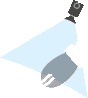
\includegraphics[scale=0.45]{sensors_r_forearm.png}}}
\put(26.4,30.9){\href{http://www.ros.org/wiki/wge100_camera}{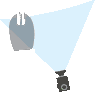
\includegraphics[scale=0.45]{sensors_l_forearm.png}}}
\end{overpic}

\subsection{Base Laser}
The base laser is a
\href{http://www.hokuyo-aut.jp/02sensor/07scanner/utm_30lx.html}{Hokuyo Top-URG
  (UTM-30LX)} scanning range finder. This laser has a 30 m and 270$^\circ$
scanning range. For more information, see the
\href{http://www.ros.org/wiki/hokuyo_node}{hokuyo\_node} package at
\href{http://www.ros.org}{ros.org}.

\subsection{Tilting Laser}
\label{tilting laser}
In addition to the base laser, the PR2 has a
\href{http://www.hokuyo-aut.jp/02sensor/07scanner/utm_30lx.html}{Hokuyo Top-URG
  (UTM-30LX)} mounted on a tilting platform located just below the pan-tilt
head. The tilting platform can sweep the scanning laser through 135$^\circ$
($+90^\circ$ and $-45^\circ$ from level) and can be controlled using the default
laser\_tilt\_controller. For more information, see the
\href{http://www.ros.org/wiki/hokuyo_node}{hokuyo\_node} and
\href{http://www.ros.org/wiki/pr2_default_controllers}{pr2\_default\_controllers}
packages at \href{http://www.ros.org}{ros.org}.

\subsection{Head Cameras}
The PR2 pan-tilt head has three cameras and a textured light projector:
\begin{description}
\label{stereo camera}
\item[Wide Stereo Camera] The wide stereo camera is part of the dual stereo pair
  and is a 100Mb color ethernet camera. The wide stereo uses the
  \href{http://www.aptina.com/products/image_sensors/mt9v032c12stc/#overview}{Aptina
    MT9V032C12STC} imager chip and has a maximum resolution of 752 x 480 pixels
  at 15 fps. The camera has a field of view (FOV) of approximately $90^\circ$
  and a 2.5mm F2.5
  \href{http://www.mars-cam.com/lenses/ccd_cmos/Technology%20Report(V-4402.5-2.5-HR).pdf}{Marshall
    V-4402.5-2.5-HR} lens. For more information, see the
  \href{http://www.ros.org/wiki/wge100_camera}{wge100\_camera} package at
  \href{http://www.ros.org}{ros.org}.

\item[Narrow Stereo Camera] The narrow stereo camera is part of the dual stereo
  pair and is a 100Mb monochrome ethernet camera.  The narrow stereo uses the
  \href{http://www.aptina.com/products/image_sensors/mt9v032c12stm/#overview}{Aptina
    MT9V032C12STM} imager chip and has a max resolution of 752 x 480 pixels at
  15 fps. The camera has a FOV of approximately $55^\circ$ and a 5.6mm F2.0
  \href{http://www.mars-cam.com/lenses/ccd_cmos/Technology%20Report(V-4405.6-2.0-HR).pdf}{Marshall
    V-4405.6-2.0-HR} lens. For more information, see the
  \href{http://www.ros.org/wiki/wge100_camera}{wge100\_camera} package at
  \href{http://www.ros.org}{ros.org}.

\item[Gigabit Ethernet Camera]
\label{ethernet camera}
The PR2 has a gigabit ethernet camera located to the left of the dual stereo
pair on the pan-tilt head.  The gigabit ethernet camera is a
\href{http://www.prosilica.com/products/gc2450.html}{Prosilica GC2450C}, which
uses the Sony ICX-625AQ imager chip and has a maximum resolution of 2448 x 2050
pixels at 15 fps.  Additionally, the gigabit ethernet camera has a 8mm F1.4-F16
\href{http://www.kowascope.com/frontend/proddetail.asp?pn=LM8JC&co=10000348}{Kowa
  LM8JC} lens. For more information, see the
\href{http://www.ros.org/wiki/prosilica_camera}{prosilica\_camera} package at
\href{http://www.ros.org}{ros.org}.

\item[Textured Light Projector]
\label{texture projector}
The PR2 has a textured light projector located to the (robot's) left of the dual
stereo pair on the pan-tilt head.  The projector has a FOV of approximately
$55^\circ$ and a 5.6mm F2.0
\href{http://www.kowascope.com/frontend/proddetail.asp?pn=LM12JC&co=10000348}{Kowa
  LM12JC} lens.  For more information, see the
\href{http://www.ros.org/wiki/pr2_camera_synchronizer}{pr2\_camera\_synchronizer} package at
\href{http://www.ros.org}{ros.org}.
Note: The projector will only work if the motors are enabled and runstop is not hit.

\end{description}

\subsection{Forearm cameras}
Each forearm of the PR2 is equipped with a 12V 100Mb color ethernet camera. The
forearm camera uses the
\href{http://www.aptina.com/products/image_sensors/mt9v032c12stc/#overview}{Aptina
  MT9V032C12STC} imager chip and has a maximum resolution of 752 x 480 pixels at
15 fps. Additionally, the forearm camera has a 2.5mm F2.0 lens.  For more
information, see the
\href{http://www.ros.org/wiki/wge100_camera}{wge100\_camera} package at
\href{http://www.ros.org}{ros.org}.

\subsection{Gripper Sensors}
\begin{description}

\item[Accelerometer] The gripper of the PR2 is equipped with a
  \href{http://www.bosch-sensortec.com/content/language1/html/3474.htm}{Bosch
    BMA150} digital triaxal accelerometer. The measurement range ($\pm$2g,
  $\pm$4g, or $\pm$8g) and bandwidth (25Hz - 1500Hz) of the accelerometer can be
  selected in software. For more information, see the
  \href{http://www.ros.org/wiki/wge100_camera}{wge100\_camera} package at
  \href{http://www.ros.org}{ros.org}.

\item[Fingertip Pressure Sensors] The default fingertips of the PR2 are sturdy
  aluminum blocks with non-slip rubber covers for added friction and compliance
  in grasping.  However, the aluminum tips can be swapped out for an (included)
  set of RoboTouch tactile sensing pads made by Pressure Profile Systems, each
  with 22 tactile sensing elements: 15 in a 5x3 array on the front surface, 2 on
  top, 2 on each side, and 1 in back, near the top.  Each tactile element has a
  pressure range of 0-30 psi (0-205 kPa) and sensitivity of 0.1 psi (0.7 kPa).
  The sensors connect to the robot via an SPI ribbon cable and two screws, and
  have a maximum scan rate of 35 Hz.

The tactile sensors are highly fragile when not protected by the rubber
covering, and so care should be taken not to damage the rubber covering.  For
more information, see the
\href{http://www.ros.org/wiki/fingertip\_pressure}{fingertip\_pressure} package
at \href{http://ros.org}{ros.org}.

\item[Calibration LED]

\end{description}

\subsection{Inertial measurement unit}
The PR2 has an inertial measurement unit (IMU) located next to the tilting
laser. The IMU is a \href{http://www.microstrain.com/3dm-gx2.aspx}{MicroStrain
  Inertial-Link 3DM-GX2} which has an accelerometer range of $\pm$5g and a gyro
range of $300^\circ/s$. For more information, see the
\href{http://www.ros.org/wiki/microstrain_3dmgx2_imu}{microstrain\_3dmgx2\_imu}
package at \href{http://www.ros.org}{ros.org}.

\subsection{Speaker}
The PR2 has one
\href{http://www.logitech.com/index.cfm/speakers_audio/home_pc_speakers/devices/199&cl=us,en}{Logitech
  V20 notebook speaker} located under the pan-tilt head next to the tilting
laser. For more information, see the
\href{http://www.ros.org/wiki/sound_play}{sound\_play} package at
\href{http://www.ros.org}{ros.org}.

\section{Power system}
\subsection{Overview}
The PR2 has a Lithium-ion (Li-ion) battery system that is charged off of a 120V
wall current. The batteries power the computers, motors, and sensors on the
robot.  Power distribution is controlled by the \emph{Power Board}, which
communicates over Ethernet to the computers in the base of the PR2.
\subsection{Power Busses}
The robot has four internal power busses:
\begin{description}
\item[AC power] The robot has a 3-prong IEC320 plug in the back of the base, which
  is connected through a circuit breaker to the four AC-DC converters used to
  charge the battery packs.  With a 120V supply, the system is designed to draw less than 15A, so a
  standard 15A or 20A outlet will suffice. The load is capable at times of
  approaching the 15A limit, make sure there are no other devices which draw
  significant power (e.g. computers or heaters) on the same circuit.
\item[Motor Power Bus] The motors get power through 3 discrete circuit breakers
  on the power board.  These create three independent motor power busses: left
  arm, right arm, and base/head.  The motor power bus can be in one of three
  states.
\begin{description}
\item[Enabled], provides a direct connection to the unregulated
  battery power. The voltage will ranges from 52V when the batteries are fully
  discharged up to 72V when connected to wall power.  i
\item[Standby], the power
  board provides a low-power 18V supply that is used for communication and
  maintaing encoder position counts.
\item[Disabled], total shut-down of the
  circuit (e.g., in the event of a major power-system problem or if manually
  disabled through the control panel).
\end{description}
\item[12V system bus] 12V power for sensors supplied by the power board. This is
  also the recommended source of power for user supplied accessories.
\item[12V computer power] 12V power for the computers supplied by the power
  board.
\end{description}
\subsection{Batteries}
The battery system has four battery bays.  Each bay is comprised of four
\href{http://www.oceanserver-store.com/18.html}{Ocean Server BA95HC-FL} 14.4V
Li-ion batteries, a
\href{http://www.v-infinity.com/adtemplate_child.asp?c=710918&p=903285&catky=764537&subcatky1=46887&subcatky2=320934}{V-INFINITY
  VF-S320-18A-CF} 18V AC-DC Power Supply, and a
\href{http://www.oceanserver-store.com/xpmibamamo.html}{Ocean Server XP-04SRW}
four-channel high current battery controller. This provides the PR2 with
approximately two hours of countinous operation after a full recharge.  For more
information, see the \href{http://www.ros.org/wiki/ocean\_battery\_driver}{ocean\_battery\_driver}
package at \href{http://www.ros.org}{ros.org}.

\subsubsection{Battery Temperature Warnings}

The PR2 battery system reports a warning in the diagnostics if the temperature goes above 50C, which is the maximum recommended operational temperature of the batteries. 

The batteries are exothermic when discharging, and tend to get hottest when they are near minimum charge. During a work day, when your PR2 is constantly charging and discharging, the temperature of the batteries can slowly climb. If your lab or workspace is warm (above 25C) you are much more likely to see this problem.

After the battery temperature goes above approximately 54C, the batteries will not charge until the battery temperature drops below 46C. 

If your batteries are reporting that they are too hot, then you need to reduce the load on the batteries. Generally, it is best to plug the robot in as soon as possible. It may take several hours for the batteries too cool down and charge.

The main power board fan will run at full power whenever the batteries are above 46C. If the fan is abnormally loud, clean your fan filter.

\subsection{Power Board}
The power board is central to the PR2's power system. This is where
the power from the batteries passes through to the rest of the
system. The power board monitors total power drawn from the batteries
by measuring the voltage and current at the power board input.

The battery power is used to provide regulated 12V to the computers and
the system bus through DC converters. Three unregulated circuits are also
provided with a unique electronic circuit breaker functionality. All outputs are
ultimately controlled by the processor located on the Power Board.

Figure~\ref{fig:power_board} shows the power board, with e-stop receiver, removed from a robot.

\begin{figure}[tb]
\centering
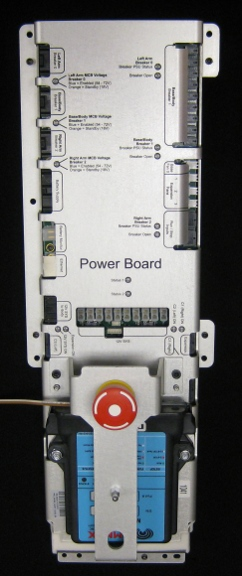
\includegraphics[scale=0.4]{pb_cropped1.jpg}
\caption{PR2 power board}
\label{fig:power_board}
\end{figure}


The Power Board contains an ARM processor with an ethernet interface. The
processor is responsible for performing a self test at power-on, monitoring the
state of all busses, providing information about the electrical system and
responding to commands. The power board is the first thing to turn on and can
not be turned off without switching off the DC circuit to the whole robot.

The power board contains many LEDs used to indicate status:
\begin{description}
\item[12V Power Bus] The LEDs in green indicate the 3 regulated 12V
  outputs are enabled and functional, shown in Figure~\ref{fig:12Vbus}.
\item[MCB Power Bus]The Blue LEDs, Figure~\ref{fig:MCBbus}, indicate
  the motor bus power is enabled. Blue indicates a voltage higher than
  the 18V standby. These LEDs can also be orange if the output state
  is in the standby state.

\item[Power Board Status]The status LEDs,
  Figure~\ref{fig:powerboardstatus}, are used by the processor for
  debugging. In the event of a failure a status code will display on
  these LEDs in the form of a number of rapid blinks followed
  by a slight pause.  Status1 indicates the location where the fault
  occured and Status2 indicates the cause of the fault.
\end{description}


\begin{figure}[htb]
\centering
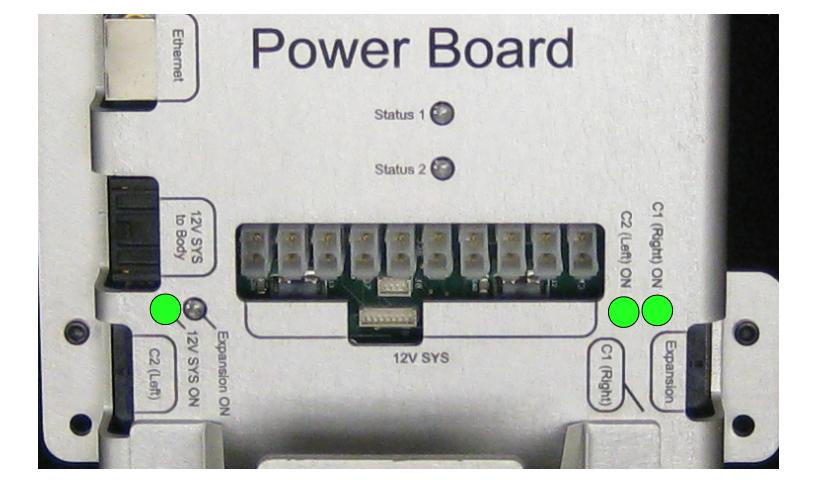
\includegraphics[scale=0.2]{pb_power1.jpg}
\caption{12V Bus Indicator LEDs}
\label{fig:12Vbus}
\end{figure}

\begin{figure}[htb]
\centering
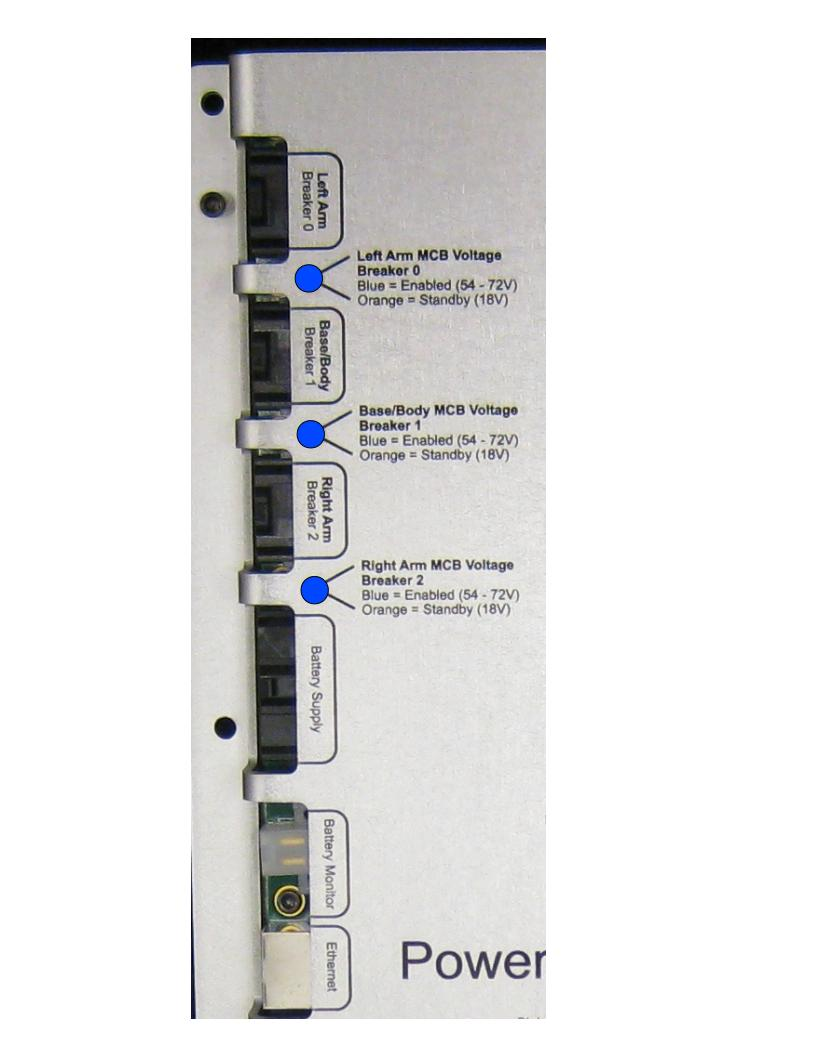
\includegraphics[scale=0.2]{pb_power2.jpg}
\caption{MCB Bus Indicator LEDs}
\label{fig:MCBbus}
\end{figure}

\begin{figure}[htb]
\centering
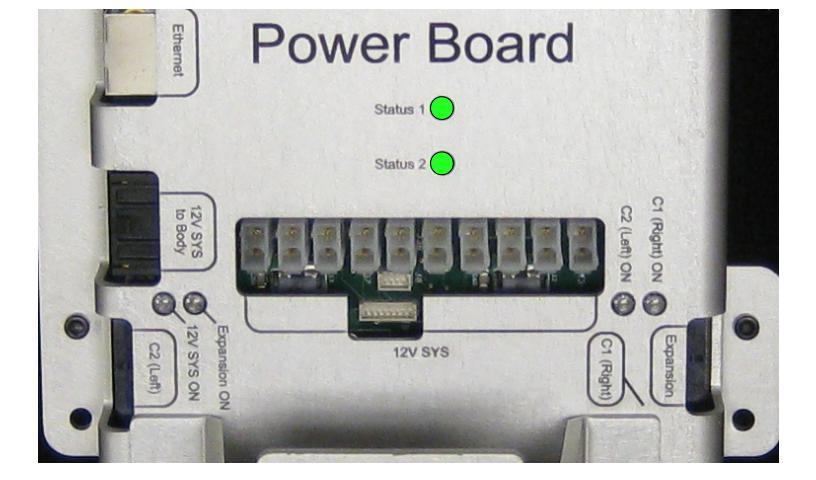
\includegraphics[scale=0.2]{pb_power3.jpg}
\caption{Power Board Status LEDs}
\label{fig:powerboardstatus}
\end{figure}


The following table decodes the meaning for the error codes. For further
diagnosis please provide the status codes in bug reports.

\begin{tabular}{|c|c|}
\hline
count & location \\
\hline
\hline
1 & Self Test \\
\hline
2 & Main Loop \\
\hline
3 & Breaker 0 \\
\hline
4 & Breaker 1 \\
\hline
5 & Breaker 2 \\
\hline
6 & Calibration Test \\
\hline
\end{tabular}

\begin{tabular}{|c|c|}
\hline
\multicolumn{2}{|c|}{Main Loop Message} \\
\hline
count &  message \\
\hline
\hline
1 & Under Voltage Lockout \\
\hline
2 & Over Temperature Lockout \\
\hline
3 & Under Current condition \\
\hline
4 & Over Current condition \\
\hline
5 & Failed Self Test \\
\hline
6 & 18v Failure \\
\hline
7 & Fan tachometer failure \\
\hline
8 & calibration CRC failure \\
\hline
9 & Battery voltage low  \\
\hline
& \\
\hline
\multicolumn{2}{|c|}{Circuit Message} \\
\hline
1 & Disable via software command \\
\hline
2 & Failed during turn on cycle \\
\hline
3 & Shutdown by E-stop \\
\hline
4 & Circuit breaker tripped  \\
\hline
\end{tabular}

\subsection {Run/Stop controls}

Besides supplying power the power board also interfaces with the wireless run/stop
radio receiver and the run/stop button. The run/stop system is
designed to reduce the power on the motor bus to a level where only the board
communications and their encoder positions are maintained. The red button and
radio system are described as provide physical run/stop control over the
motors in the robot. This mechanism is
implemented in hardware and can not be altered by software.

Please note that the run/stop system only reduces power to the motor power bus
and nothing else. If there is an electrical problem or power needs to be
shutdown for service, the red DC circuit breaker on the rear lower panel is the
only way to totally shut off the power board.


\subsection{Power for sensors}
The power board provides a \emph{12V system bus}, that
provides a well regulated 12V supply. The regulated 12V supply is the only
supply designed for additions and expansion. This 12V supply is essentially
always on once the Power Board completes its self test. It is also monitored for
undervoltage conditions.

THe 12V use supply powers various electronics devices in the robot, including both Hokuyo scanners, the ethernet switches, the wireless
AP, and the run/stop receiver.  There is 5A of
additional capacity available for expansion.

Access to the 12V accessory bus is available in several locations:\\

Inside the top head assembly.\\

{\bf insert picture}\\


In the upper back.\\

{\bf insert picture}\\


In the lower back, directly connecting to the power board.\\

{\bf insert picture}\\

The robot electrical systems are complex, and it is easy to damage robot components
by hot-plugging.  Never plug in or unplug any components inside the robot unless
the power system is shut off completely.

All 12V connectors in the robot use the same connector, a 2x1 Molex Mini-Fit
Jr. The mating connector part number is {\bf 39-01-3022} or from Digikey {\bf
  WM1021-ND}. Pin one is negative and pin 2 is positive. Pin 2 is the pin
closest to the latch.


